\documentclass{article}
\usepackage{graphicx} % Required for inserting images
\usepackage{amsmath}

\title{\textbf{Expectations vs Reality: AI for Learning}}
\author{Group 13}
\date{\today}

\begin{document}

\maketitle

\section{Introduction}
\subsection{Group Info}

\begin{itemize}
    \item Group Number: 13
    \item Abdur Rehman Tariq, CMSID: 623486
    \item Muhammad Asad Rehman. CMSID: 585237
    \item Ahmad Hamza, CMSID: 623320
\end{itemize}




\section{Project Overview}
People have many grievances about AI when used for learning: wrong outputs, hallucinations, and lengthy gibberish are among a few \cite{gokcearslan2024chatbots}. We decided to ask people about common problems they face when using AI (particularly LLMs) in educational settings \cite{chen2020ai} and then Benchmark the Most commonly used models against AMC Maths Problems \cite{berkeley2025math}. Doing so allows us to investigate if there exists a gap between actual benchmark results and users' predicted results \cite{katsantonis2024students}. 

\section{Methodology}
We collected responses about common AI faults via a Microsoft form and a separate form was made to test the LLM’s. The LLM form was based on AMC maths problems (the kind used in actual AI benchmarks) that tested logical and spatial reasoning in a variety of ways. The “human” form was used to gauge peoples  methodology when using AI, their most frequently used models and what issues they faced. It finally ended with a very simple question that anyone should have been able to solve. However, we weren't looking for the answer, we were testing to see if people were willing to solve the question at all.

\section{Key Findings}
\subsection{User Expectations: Human Form Analysis}
Based on the results of the Human form, we were able to conclude that people used the following models the most:

\begin{table}[h!]
\centering
\begin{tabular}{|l|c|c|}
\hline
\textbf{Name} & \textbf{n} & \textbf{Count \% of answered (n)} \\ \hline
ChatGPT & 31 & 66.0\% \\ \hline
Gemini & 24 & 51.1\% \\ \hline
Claude AI & 13 & 27.7\% \\ \hline
Meta AI & 1 & 2.1\% \\ \hline
\end{tabular}
\caption{Model Response Analysis}
\label{tab:model_analysis}
\end{table}


\begin{figure}[htbp]
    \centering
    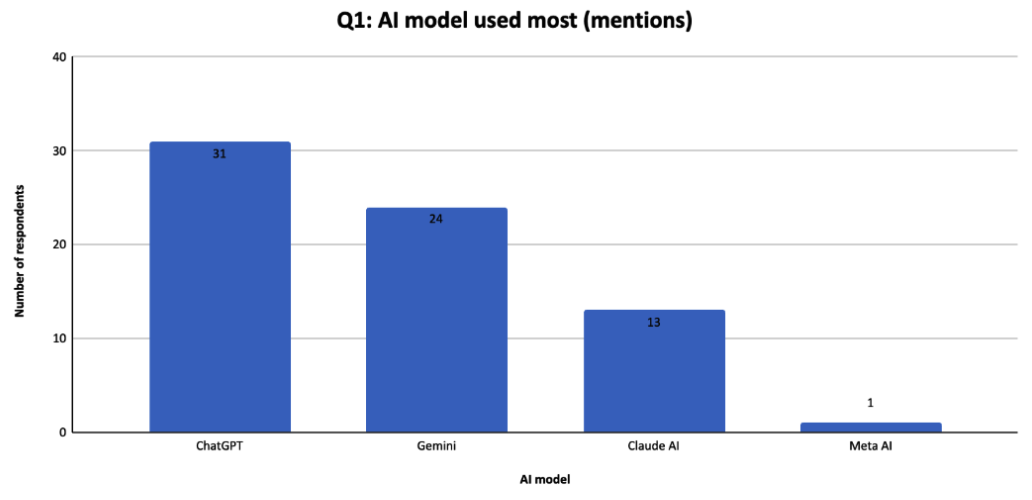
\includegraphics[width=0.8\textwidth]{graph.png}
    \caption{Most used model frequency count}
    \label{fig:Bar Chart}
\end{figure}

Using the Equation: 
\begin{equation}
    \text{Model Percentage Use} = \frac{\text{Model Response Count}}{47} \times 100
    \label{eq:model_percentage}
\end{equation}


We calculated the percentage of respondents who used each model which helped us decide what niche and most used models to target. 


Particularly Deepseek which none of the respondents seemed to use as can be seen in 
\textbf{Table~\ref{tab:model_analysis}} and \textbf{Figure~\ref{fig:Bar Chart}}

\subsection{LLM Benchmark Analysis}
In contrast, we tested and then calculated the average score for the LLM Benchmark form which totaled to an impressive 5.8/6 across the 5 tested models:



Using the model Percentages (See Equation \ref{eq:model_percentage} for details.)

We bench marked the models against 7 AMC Maths problems which resulted in the following Average performance/scores:

\begin{table}[h!]
\centering
\caption{Model Rankings \& Categorization}
\label{tab:model_rankings}
\resizebox{\textwidth}{!}{%
\begin{tabular}{|l|l|c|c|c|}
\hline
\textbf{Model Name} & \textbf{Model Tier} & \textbf{Score (Max 7)} & \textbf{Accuracy Rate} & \textbf{Completion Time (s)} \\ \hline
GPT 6.1 Sol & Frontier / High-Reasoning & 7 & 100.0\% & 87 \\ \hline
Deepseek V4.1 Flash & Frontier / High-Reasoning & 7 & 100.0\% & 223 \\ \hline
Gemini 3.8 Flash & Mid-Tier / Generalist & 6 & 85.7\% & 126 \\ \hline
Claude Sonnet 5.5 & Mid-Tier / Generalist & 5 & 71.4\% & 81 \\ \hline
Perplexity Sonar Pro & Search / Specialized & 4 & 57.1\% & 83 \\ \hline
\textbf{Average / Total} & \textbf{—} & \textbf{5.8} & \textbf{82.9\%} & \textbf{120.0} \\ \hline
\end{tabular}%
}
\end{table}





\section{Conclusion and Recommendations}
In conclusion, there is an obvious gap between the actual AI output and what people expect from it. This could be improved by targeting niche models (like Deepseek which performed the best) and educating the average user about prompt engineering techniques.


\bibliographystyle{plain}
\bibliography{references}



\end{document}
